After computing the correlators $\ct$, we used them to calculate $\DEt$ (equation \ref{eqn:energy}) and $\matb$ (equation \ref{eqn:matelem}). This is when we had to consider two additional conditions: firstly, the observables are decorrelated on Markovian time but correlated on physical time; secondly, because of the exponential problem, as $\t$ grows so does the error, rendering later time calculations useless.

The physical time correlation is relevant because the energy gap, which is used itself to compute the matrix element,  is a
function of $\ct$, $\ctm$ and $\ctp$: we dealt with it applying the Jackknife method to resample the observables and automate the
statistical analysis for correlated variables. Regarding the exponential problem, we set a cutoff of $20\%$ to the relative error of each energy gap and matrix element value; only the surviving values were kept and used for the analysis.

In figure \ref{fig:energyA3} we show the $20$ surviving values of the energy and their error. Figure \ref{fig:matA3} does the same for the $15$ matrix elements.
%--------------------------------------
\begin{figure}[H]
  \centering
  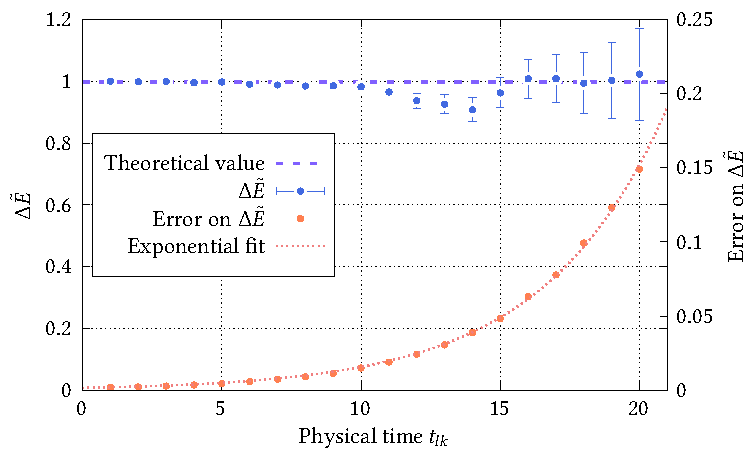
\includegraphics[width=\linewidth]{deltae}
  \caption{\label{fig:energyA3}In blue, energy gap from $\ct$ for different physical times; in orange, its error. The exponential growth of the error
  is highlighted.}
\end{figure}


\begin{figure}[H]
  \centering
  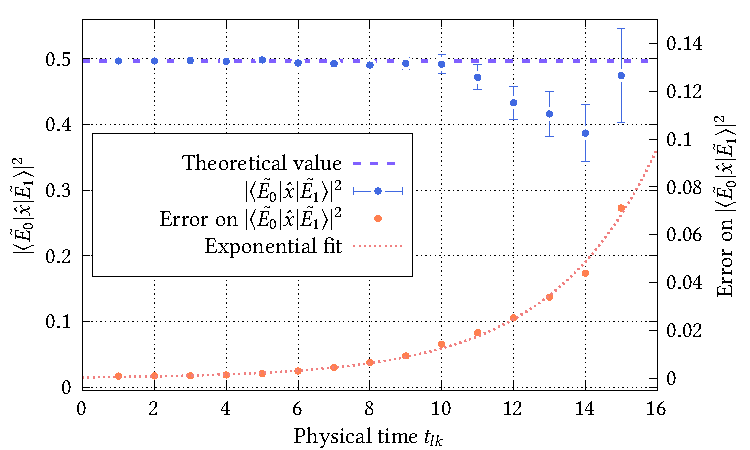
\includegraphics[width=\linewidth]{matelem}
  \caption{\label{fig:matA3} In blue, matrix element from $\ct$ for different physical times, the error bars are doubled to improve visibility; in orange, its error. The exponential growth of the error
  is highlighted.}
\end{figure}
%------------------------------------
The best estimates for $\DEt$ and $\matb$ are the weighted mean of the values that survive the cutoff and are collected in tables \ref{tab:energyresults} and \ref{tab:matrixresults}. The data shown in the figures correspond to the $A3$ lattice of table \ref{tab:alllattices}, which collects
the parameters of the five lattices that were used in the simulation.
% -----------------------------------------
\begin{table}[h!]
\centering
\begin{tabular}{@{}ccccc@{}}
\toprule
Lattice & $N$    & $a$      & $D_{bin}$ & $N_{bin}$ \\ \midrule
$A1$    & $64$   & $1$      & $50$      & $20000$   \\
$A2$    & $128$  & $0.5$    & $500$     & $10000$   \\
$A3$    & $256$  & $0.25$   & $500$     & $10000$   \\
$A4$    & $512$  & $0.125$  & $1000$    & $2000$    \\
$A5$    & $1024$ & $0.0625$ & $3000$    & $2000$    \\ \bottomrule
\end{tabular}
\caption{Parameters used for the different lattices.}
\label{tab:alllattices}
\end{table}
%---------------------------------------
\\
We kept the physical parameters $m=1$, $\w=1$, $Na=64$ fixed and repeated this procedure for each lattice of table \ref{tab:alllattices}. The more sites a lattice has, the higher the amount of values that survive the $20\%$ relative error cutoff: from lattice $A1$ to $A5$ we were able to work with a number of data in the order of $5$, $10$, $20$, $40$, $80$.
The results are collected in table \ref{tab:energyresults} for the energy gaps and table \ref{tab:matrixresults} for the matrix elements;
the theoretical values correspond to equation \ref{eqn:phys1} for $\DEt$ and equation \ref{eqn:phys2} for $\matb$.
%-------------------------------------------------------------------------------
\begin{table}[h!]
\centering
\begin{tabular}{@{}ccc@{}}
\toprule
Lattice              & \multicolumn{2}{c}{$\Delta\tilde{E}$} \\ \midrule
                     & Theoretical       & Obtained          \\
$A1$                 & $0.9624$          & $0.9634(17)$      \\
$A2$                 & $0.9899$          & $0.9887(13)$      \\
$A3$                 & $0.9974$          & $0.9970(11)$      \\
$A4$                 & $0.99935$         & $1.0002(6)$       \\
$A5$                 & $0.9998$          & $0.9993(5)$       \\ \bottomrule
\end{tabular}
 \caption{Energy gaps for the $5$ lattices.}
 \label{tab:energyresults}
\end{table}
%-----------------------------------------------------------------------------
\begin{table}[h!]
  \centering
\begin{tabular}{@{}ccc@{}}
\toprule
Lattice & \multicolumn{2}{c}{$\matb$}           \\ \midrule
                     & Theoretical       & Obtained          \\
$A1$                 & $0.4472$          & $0.4477(7)$       \\
$A2$                 & $0.4851$          & $0.4850(5)$       \\
$A3$                 & $0.4961$          & $0.4965(5)$       \\
$A4$                 & $0.4990$          & $0.4991(3)$       \\
$A5$                 & $0.4998$          & $0.4999(3)$       \\ \bottomrule
\end{tabular}
\caption{Matrix elements for the $5$ lattices.}
\label{tab:matrixresults}
\end{table}
